\clearpage
\begin{flushright}
	\textit{Лекция №13}
	\textit{2015.10.27}
\end{flushright}


Осуществляется переход в режим ядра при захвате и освобождении семафора, т.е. происходит переключение контекста.
Считающие семафоры могут принимать не отрицательные значения. Современные ОС поддерживают наборы считающих семафоров. По своей семантике наборы семафоров похожи на массивы (массивы семафоров). У набора семафоров есть важное свойство: одной неделимой операцией можно изменить значения всех семафоров или части семафоров.
Если процесс использует большое кол-во разных семафоров то сложно уследить за состоянием семафоров, то такие программы могли висеть в тупиках.

Другие средства взаимоисключения: мьютекс.

\section{Мьютексы}

Между семафорами и мьютексами есть серьезные различия:
\begin{enumerate}
    \item Мьютекс имеет хозяина, только процесс, захвативший мьютекс, может его освободить. Семафор может освободить любой другой процесс, зная идентификатор.
    \item Чтобы обеспечить для мьютекса свойство владельца, если мьютекс пытается захватить более приоритетный процесс, то временно повышается приоритет процесса хозяина.
    \item Мьютекс не может быть случайно удален, т.е. если он захвачен кем то, то удалить процесс–хозяин – нельзя. 
\end{enumerate} 

\section{Задача обедающих философов}

\begin{figure}[H]
    \centering
    
\includegraphics[width=\textwidth]{pic/1.png}
    \caption{pic}
\end{figure}

Возможны три сценария действия философов (эти ситуации – негативные в системе):
\begin{enumerate}
    \item Голодание: Каждый пытается взять левую и правую вилку, если удается, то он начинает есть. Через какое то время кладет вилки обратно.
    \item Тупик: Философ берет правую вилку, удерживает её и пытается взять левую.
    \item Зависание: Философ берет правую вилку, если не может взять левую , то кладет обратно. Захват и освобождение одних и тех же ресурсов. Это похоже на трешинг – загрузка и выгрузка одних и тех же страниц.
\end{enumerate} 


\begin{figure}[H]
    \centering
    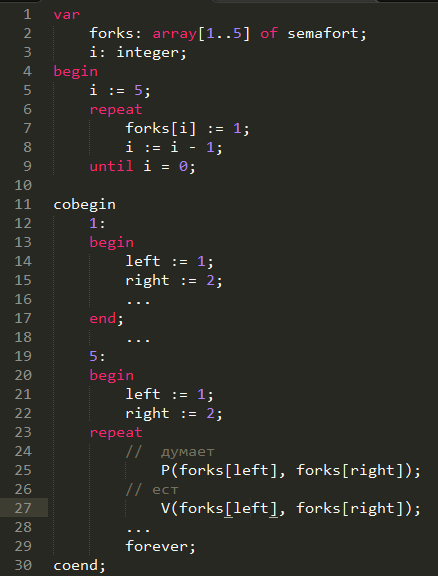
\includegraphics[width=\textwidth]{listing/1.png}
    \caption{listing}
\end{figure}

\section{Задача производство потребление}

Один процесс производит данные, другой процесс – считывает эти данные. Один – кладет произведенные данные в ячейки буфера, другой – считывает из ячеек буфера.  Дейкстра предложил решение на трех семафорах, двух считающих и одном бинарном. 

$SB$ – бинарный семафор.\\
$SE$ – считает пустые ячейки.\\
$SF$ – число заполненных ячеек.

\begin{figure}[H]
    \centering
    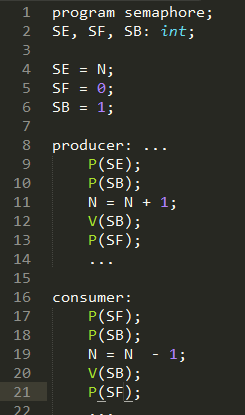
\includegraphics[width=\textwidth]{listing/2.png}
    \caption{listing}
\end{figure}

Если покупатель работает быстрее, то покупатель будет блокирован на SF, так как нет заполненых ячеек.\\
Если продавец работает быстрее, то при попытке декрементировать SE, продавец будет блокирован.  Изменение N – критическая секция. \\
Дейкстра решил с использованием отдельных семафоров. Но так же можно решить с помощью набора семафоров.

\section{Мониторы}

Язык параллельного программирования: Ада. 

Цель монитора – структурировать средства взаимоисключения.

Идея – создание механизма, который бы соответствующим образом унифицировал взаимодействие параллельных процессов. Монитор представляет синтаксическую конструкцию. Монитор содержит данные и процедуры, которые могут изменять эти данные. Говорят, что монитор защищает свои данные, так как изменить данные монитора можно только с помощью процедур монитора. Монитор может предоставляться языком, а может быть системным средством. Монитор гарантирует, что в каждый момент времени процедуры монитора могут использовать только один процесс. Если процесс успешно вызвал процедуру монитора, то говорят, что такой процесс находится в мониторе, остальные процессы ставятся к монитору в очередь. Классические мониторы используют 2 системных вызова wait и signal, эти системные вызовы определены на переменной типа «условие».

Рассмотрим пример простого монитора, потом кольцевого, а потом монитор Хоара (читатели-писатели).

\subsection{Простой монитор} – обеспечивает выделение единственного ресурса произвольному числу процессов. \cite{C_Deitel2}

\begin{figure}[H]
    \centering
    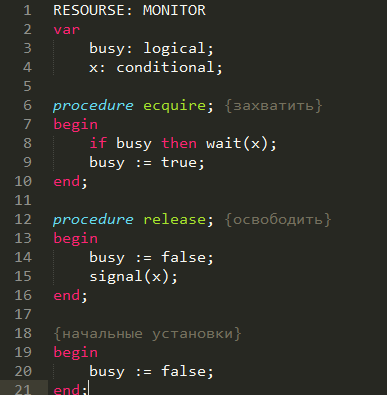
\includegraphics[width=\textwidth]{listing/3.png}
    \caption{listing}
\end{figure}

Монитор обслуживает произвольное число процессов, кол-во которых ограничено длинной очереди.  
\verb|signal(x)| проверяет очередь процессов к монитору и выбирает один для запуска на выполнение.

\subsection{Монитор кольцевой буфер}

Также задача производство потребление.
Понятие синхронизация процессов – связана с выравниванием скоростей на каком то отрезке деятельности. 
Взаимоисключение процессов - ???.

\begin{figure}[H]
    \centering
    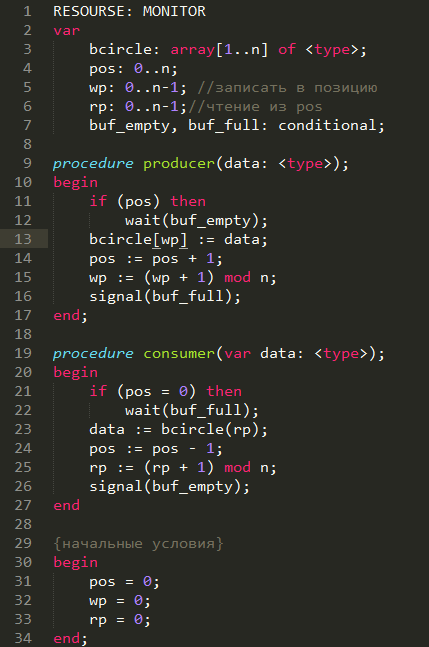
\includegraphics[width=\textwidth]{listing/4.png}
    \caption{listing}
\end{figure}

Механизм кольцевого буфера используется для организации работы spooler. SPOOL – Simultaneous Peripheral Operations On Line – для вывода текста на принтер.  

